% Matteo Veneziano -- Solid State Physics Formula Sheet
\graysec{Réseaux cristallins dans l'éspace réel et réciproque}
\begin{squishlist}
    \item Énergie électrost.\ $E = - M_d \frac{e^2}{4\pi \varepsilon_0 a}$ \textbf{Cst de Madelung} specif.\ pour une struct.\ donnée
    \item \textbf{Liaison covalente}: partage d'\elec entre les atomes, favorable en présence d'orbitales de valence partiell.\ remplies. E.g.\ diamant, hybridisation $sp^3$ $\Rightarrow$ nb de coordin.\ 4 \\
    \textbf{Liaison ionique}: entre atome avec un seul \elec de valence et un qui manque d'un \elec de valence. Resulte en deux ions avec couches completes.
    \item Taux de remplissage $t$: rapp.\ entre le volume occupé par les atomes (assimilés à des sphères dures de rayon $r$) et le volume de la maille considérée
\end{squishlist}
\graypar{Réseaux cristallins}
\begin{squishlist}
    \item $\vec{R} = \sum_{j=1}^{3} n_j \vec{a}_j$ un vecteur du \textbf{réseau de Bravais (RB)} (réseau de points)
    \item Une \textbf{cellulle (ou maille) primitve} est un volume d'espace qui, translaté par les vecteurs $\vR$ du RB, remplit exactement l'espace sans recouvrement. Ne contient qu'un point du RB, donc a volume $v = 1/n$ avec $n$ la densité de points du RB.
    \item La \textbf{cellule de Wigner-Seitz} est la région de l'espace qui est plus proche à un point du RB que de n'importe quel autre point. On l'obtient en tracant les plans bissecteurs des ligne qui connectent les points.
    \item Une \textbf{structure cristalline} est un RB avec une base formée de un ou plus atomes
    % \begin{minipage}{.25\columnwidth}
        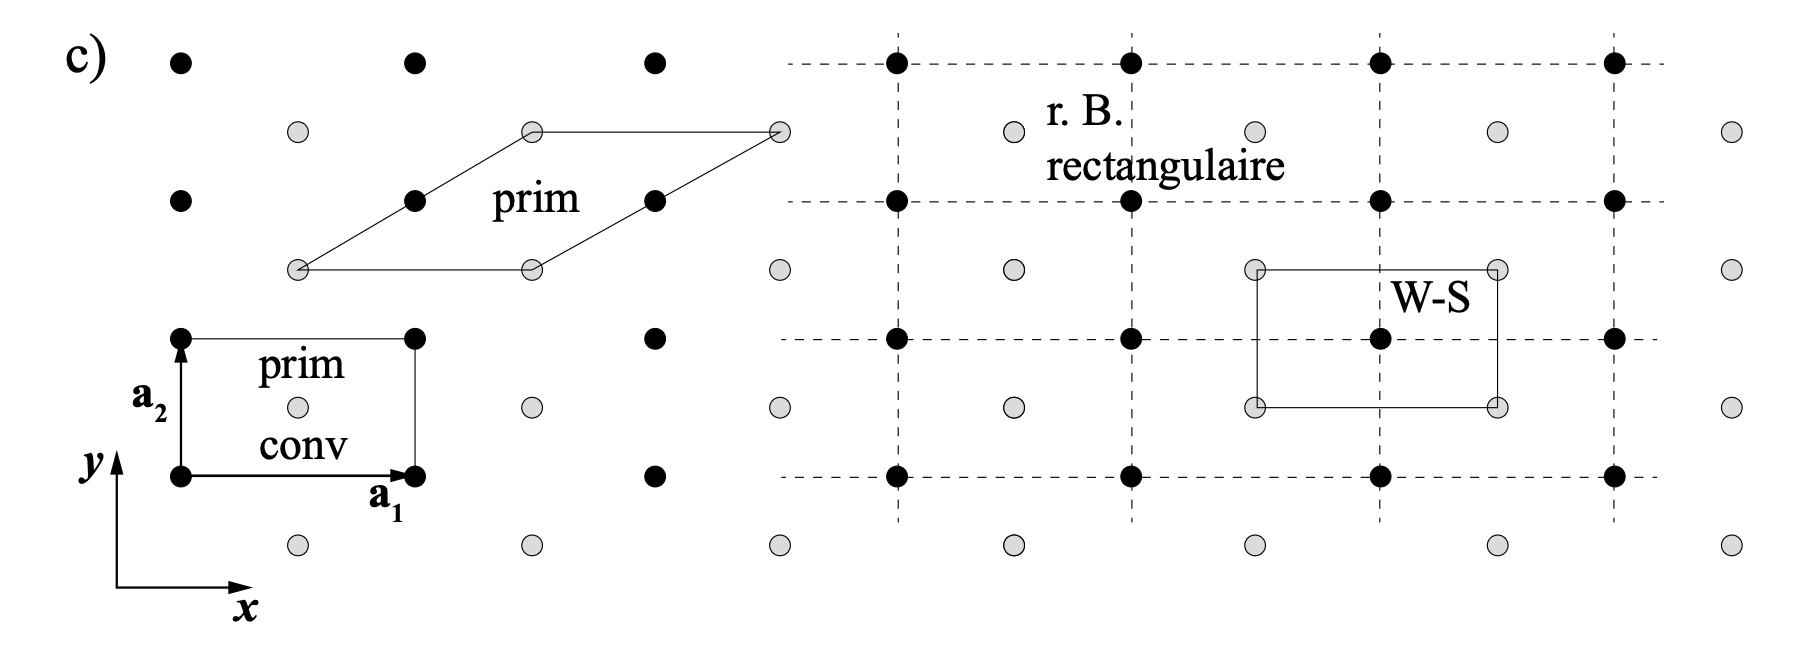
\includegraphics[width=0.6\columnwidth]{figures/structure-exemple.png}
    % \end{minipage}
    \item Le \textbf{réseau réciproque} (RR) est formée des $\vG$ t.q.\ $\exp(i \vG \cdot \vR) = 1$ \\
    $\vG = \sum_{i=1}^{3}h_i \vec{b}_i $\squishsep $\vec{a}_i \cdot \vec{b}_j = 2 \pi \delta_{ij}$ \squishsep $\vec{b}_1 = 2 \pi \frac{\vec{a}_2 \times \vec{a}_3}{\vec{a}_1 \cdot (\vec{a_2 \times \vec{a}_3})}$ et perm.\ cycl.\ 
    \item Le volume d'une cell.\ prim.\ du réseau réciproque est $\vec{b}_1 \cdot (\vec{b}_2 \times \vec{b}_3) = \frac{(2\pi)^3}{v} = \frac{(2\pi)^3}{V/N}$
\end{squishlist}    

\graypar{Zones de Brillouin}
\begin{squishlist}
    \item La \textbf{1ère zone de Brillouin (1ZDB)} est la cellule de Wigner-Seitz du réseau réciproque. La \textbf{nième zone de Brillouin (nZDB)} est l'ensemble des points atteints à partir de l'origine en traversant $(n-1)$ plans de Bragg
    \item Le volume de la nZDB est égal à celui de la 1ZDB. On peut par translations de vecteur $G$ réduire une ZDB à la 1ZDB (passage d'une description en schéma de zone étendue à une de zone réduite).
\end{squishlist}

\graypar{Détermination de la structure cristalline}
Techn.\ expérim.\ pour déterminer la struct.\ cristalline: diffraction de rayons X.
\begin{squishlist}
    \item \textbf{Théorie de Bragg:} les rayons X sont réfléchis par les plans atomiques du cristal. \textbf{Condition de Bragg:} $n \lambda = 2d \sin \Theta$, $n \in \mathbb{N}$ (interférence constructive d'ondes émerg.\ de plans successifs). $\lambda < 2d$. \quad
    \textbf{Condition de Laue:} $\vec{K} = \vk'-\vk = \vG$

    \item \textbf{Indices de Miller:} les plans du réseau sont caractérisés par $(h,k,l)$. $(h,k,l)$ intersectent les axes $x,y,z$ en $1/h,1/k,1/l$.\\
    $\vG = h \vec{b}_1 + k \vec{b}_2 + l \vec{b}_3$ vec du RR perp.\ à la famille de plans, avec plus petite norme $G_{\min} = 2\pi / d \quad G = n G_{\min}$
\end{squishlist}

\graysec{Dynamique du réseau. Notion de phonon}
\begin{squishlist}
    \item \textbf{Approximation harmonique}: on néglige termes super.\ à 2
    \\ \textbf{Approximation adiabatique:} les vitesses \elec sont de l'ordre de la vit.\ de Fermi ($\sim 10^8$ cm/sec) et la vitesse thermique des ions est plus faible $\Rightarrow$ les \elec suivent instantanément le mouvement des ions. Les \elec se trouvent tousjouts dans l'état fondamental correspondant à la configuration ionique.
    \item $u$ amplitude de déplacement
\end{squishlist}

\graypar{Modes normaux d'un RB monoatomique 1D}
\begin{squishlist}
    \item Chaine linéaire d'ions de masse $M$ séparés à l'ex.\ par $a$ ($R = na$)\\
    $U_{\text{harm}} = \frac{1}{4} \sum_{n,n'} C_{n,n'}(u_n - u_n')^2 \quad C_{n,n'} = C_{n',n} = \phi_{xx}(na - n'a)$
    % \item Interactions entre plus proches voisins: les seuls coefs non nuls sont t.q.\ $n-n'= \pm 1$
    \item \textbf{Conditions de Born von Karman:} $u_{N+1} = u_1 \Longrightarrow U_{\text{harm}} = \frac{1}{2}\sum_{n=1}^{N}C(u_{n+1}-u_n)^2$
    \item $H(p,u) = \sum_{n=1}^{N}\frac{p^2_n}{2m} + \frac{C}{2}\sum_{n=1}^{N}(u_{n+1} - u_n)^2 \Longrightarrow \ddot{u}_n = -\frac{C}{m}(-u_{n-1}+2u_n - u_{n+1})$
    \item $u_n(t) = \frac{1}{\sqrt{N}} \sum_{\nu=0}^{N-1}a_{\nu} \exp[ i (k_{\nu}na - \omega_{\nu}t)] + c.c.$ \quad $k_{\nu} = \frac{2\pi \nu}{aN} \quad \nu = 0,1,\ldots, N-1$ 
    \item $\omega_{\nu} = 2 \sqrt{\frac{C}{m}} \left| \sin \frac{k_{\nu}a}{2}\right|$ \textbf{Courbe de dispersion} (linéaire pour $k$ faible par rapport à $\pi/a$)

    \squishline

    \textbf{3D}
    \item $u_{\alpha}(\vR) = \frac{1}{\sqrt{3N}}\sum_{\nu}\sum_{s=1}^{3} a_{\nu,s} \varepsilon_{\alpha,s}(\vk_{\nu}) \exp [i \vk_{\nu} \cdot \vR - i \omega_s(\vk_{\nu}t)] + c.c.$ \\ 
    Pour chacune des $N$ (nb de mailles) valeurs $\vk_{\nu}$ dans la 1ZDB, 3 directions $\vec{\varepsilon}_s$ de polarisation, donc $3N$ modes propres

\end{squishlist}

\graypar{Modes normaux d'un RB 1D avec une base, $N$ mailles}
\begin{squishlist}
    \item $U_{\text{harm}} = \frac{K}{2}\sum_{n=1}^{N}(u_n - v_n)^2 + \frac{G}{2} \sum_{n=1}^{N} (u_n - v_{n-1})^2$ \quad \textbf{2 ress.\ différents, même masse}
    \item $\left\{ \begin{aligned}
        & m\ddot{u}_n = -K (u_n - v_n) - G(u_n - v_{n-1}) \\
        & m\ddot{v}_n = K (u_n - v_n) + G(u_{n+1} - v_{n})
    \end{aligned}\right.
    \Rightarrow 
    \left\{ \begin{aligned}
        & u_n = \sum_{\nu = 0}^{N-1} a_{\nu} \exp (i k_{\nu}na - i\omega_{\nu}t) + c.c \\
        & v_n = \sum_{\nu = 0}^{N-1} b_{\nu} \exp (i k_{\nu}na - i\omega_{\nu}t) + c.c
    \end{aligned}\right.$

    \item $\omega_{\nu}^2 = \frac{K+G}{m} \pm \frac{1}{m}\sqrt{(K+G)^2 - 4KG \sin^2 \frac{k_{\nu}a}{2}} \qquad \frac{a_{\nu}}{b_{\nu}} = \mp \frac{K + G\exp(ik_{\nu}a)}{|K + G\exp(ik_{\nu}a)|}$
    \item Au bord de 1ZDB, si $K > G \quad \Longrightarrow \quad \omega_{\text{opt}}= \sqrt{\frac{2K}{M}} \quad \omega_{\text{acous}} = \sqrt{\frac{2G}{M}}$ \\
    \item Pour chacune des $N$ valeurs de $k$ il y a 2 solutions $\Rightarrow 2N$ modes normaux de vibrations. Branche inférieure (\textbf{acoustique}, déplacement en phase, dynamique dominée par interactions entre cellules) et supérieure (\textbf{optique}, les ions d’une même cellule vibrent l’un par rapport à l’autre,).
    \item Dans le cas \textbf{à 3 dimensions:} pour une cellule primitive avec une base de $p$ atomes, $3N$ modes acoustiques et $(3p - 3)N$ modes optiques de vibrations.
    
    \squishline

    \textbf{2 masses, même ressort}
    \item $\omega^2(k) = K \left(\frac{1}{M_1}+\frac{1}{M_2}\right) \pm K \sqrt{\left(\frac{1}{M_1}+\frac{1}{M_2}\right) - \frac{4}{M_1 M_2} \sin^2(ka/2)}$
    \item Au bord de 1ZDB, si $M_1 > M_2 \quad \Longrightarrow \quad \omega_{\text{opt}}= \sqrt{\frac{2K}{M_2}} \quad \omega_{\text{acous}} = \sqrt{\frac{2K}{M_1}}$ \\
    La largeur de la bande interdite (gap) entre branches acoustiques et optiques se réduit lorsque les deux masses d’un système sont similaires.
\end{squishlist}

\graypar{La notion de phonons}
\begin{squishlist}
    \item La contribution à l'énergie totale d'un mode normal de fréquence $\omega_s(\vk_{\nu})$ est $\left( n_{\vk_{\nu,s}} + \frac{1}{2}\right) \hbar \omega_s(\vk_{\nu})$ \qquad $n_{\vk_{\nu,s}} = 0,1,2,\ldots$ \textbf{nb d'occupation} du mode normal $\nu,sd$
    \item On passe à une déscript.\ corpusculaire: nb $n_{\vk_{\nu,s}}$ de \textbf{phonons} de vecteur d'onde $\vk_{\nu}$ et polar.\ $s$ dans le crystal.
    Les phon.\ d'un rés.\ ne port.\ pas de quant.\ de mouv.\

    \item Lors de l’inter.\ entre une particule incid.\ dans le cristal et les phon.\, tout se passe comme si une pseudo quant.\ de mouvem.\, $\hbar \vk$ (crystal momentum), était conservée à un vecteur $\hbar \vG$ du réseau réciproque près. \\
    $\vec{p} + \sum_{\nu,s}\hbar \vk_{\nu}n_{\vk_{\nu,s}} = \vec{p}' + \sum_{\nu,s}\hbar \vk_{\nu}n'_{\vk_{\nu,s}} + \hbar \vG$ \qquad \\
    $E + \sum_{k_{\nu},s} \hbar \omega_s (\vk_{\nu}) n_{\vk_{\nu},s} = E' + \sum_{k_{\nu},s} \hbar \omega_s (\vk_{\nu}) n'_{\vk_{\nu},s}$
    % \end{minipage}

    \item \textbf{Diffusion à un phonon:} $\frac{p'^2}{2m} = \frac{p^2}{2m} + \hbar \omega_s \left( \frac{\vec{p'}-\vec{p}}{\hbar}\right)$
    
\end{squishlist}

\graysec{Propriétés thermiques en relation avec les phonons}
\begin{squishlist}
    \item $c_v = \left.\D{T}{u}\right|_V$ chaleur spécifique du réseau
    \item \textbf{Loi de Dulong et Petit:} $c_v = 3n k_B$ ($n$ densité d'atomes). En accord avec les mesures pour une bonne partie des solides et proches de la température ambiante.
    \item $u = \frac{1}{V} \sum_{\vk,s} \hbar \omega_s(\vk) \left( \braket{n_{\vk,s}}+\frac{1}{2}\right)$ \quad $\braket{n_{\vk,s}} = \frac{1}{\exp[\beta \hbar \omega_s(\vk)]-1}$ (Bose-Einstein) \\
    À haute $T$, si $x = \frac{\hbar \omega_s}{k_B T}$, \quad $\braket{n_{\vk,s}} \approx \frac{1}{x} - \frac{1}{2} + \frac{x}{12} \approx \frac{k_BT}{\hbar \omega_s} - \frac{1}{2}$
    
    \item \textbf{Expression génerale:} $c_v = \D{T}{} \sum_s {\displaystyle\int_{\text{1ZDB}}} \frac{\ud^3 k}{(2\pi)^3} \frac{\hbar \omega_s(\vk)}{\exp[\hbar \omega_s(\vk)/k_B T]-1}$
    
    \squishline

    \textbf{Limites }
    \item \textbf{Haute temperature:} Pour $\hbar \omega_s(\vk)/k_BT \ll 1$ on retrouve D\&P
    \item \textbf{Basse temperature:} À basse $T$ les modes tels que $\hbar \omega_s(\vk) \gg k_BT$ donnent une contribution négligeable (e.g. les modes optiques). Par contre modes acoustiques non-négligeables car $\omega_s(\vk) \rightarrow 0$ lorsque $k \rightarrow 0$ $\Longrightarrow$ $c_v = \frac{2\pi^2}{5}k_B \left(\frac{k_B T}{\hbar c}\right)^3 \propto T^3$
    
    \squishline

    \textbf{Entre les domaines de hautes et basses température}

    \item \textbf{Modèle d'Einstein:} on fait l'hypothèse que la rélation de dispersion $\omega_s(\vk)$ est const \\
    $u = 3 \frac{N}{V} \braket{n_E}\hbar \omega_E = 3n \frac{\hbar \omega_E}{\exp[\hbar \omega_E/k_BT]-1} \Longrightarrow c_v = 3nk_B \left(\frac{\hbar \omega_E}{k_BT}\right)^2 \frac{\exp[\hbar \omega_E /k_BT]}{(\exp[\hbar \omega_E /k_BT] - 1)^2}$ \\
    Pas de modes qui peuv.\ être excités à basse $T$ $\rightarrow$ $c_V$ décroit trop vite en descend.\ $T$

    \item \textbf{Modèle de Debye:} (1) on remplace toutes les branches du spectre de vibration par 3 branches ayant la même relation de dispersion $\omega = c|k|$ ($\omega \propto \sqrt{C/m}|k|$) \\
    (2) on remplace l'intégrale sur 1ZDB par une int.\ sur une sphère de rayon $k_D$, de telle sorte que la sphère contienne $N_{\text{atomes}}$ vecteurs d'onde: \\
    $\left( \Omega_{\text{Debye}} \right) \cdot \text{densité de }k = \# \text{nb atomes}\quad \text{densité}=\frac{\text{vol.\ du cristal}}{\text{volume d'un }k}$ e.g.\ $\frac{N a^2}{(2\pi)^2}$ en 2D \\
    $\Longrightarrow$ en 3D $n = \frac{N}{V} = \frac{k_D^3}{6\pi^2}$
    \item En définissant $\omega_D = ck_D$ et $k_B \theta_D = \hbar \omega_D$ ($T > \theta_D$: tous les modes commencent à être excités) on a
    $c_v = 9 n k_B \left(\frac{T}{\theta_D}\right)^3 {\displaystyle \int_0^{\theta_D/T}} \frac{x^4 e^x}{(e^x - 1)^2} \ud x$ où $x = \beta \hbar c k$
    \item \textbf{Basse temperature}($T/\theta_D \ll 1$): $c_v = \frac{12\pi^4}{5} n k_B \left( \frac{T}{\theta_D}\right)^3 \propto T^3$
    \item \textbf{Haute temperature:}($T/\theta_D \gg 1$) on retrouve D\&P
\end{squishlist}

\graypar{Densité de modes en $\omega$}
\begin{squishlist}
    \item $g(\omega) \ud \omega = \frac{\ud^n k}{(2\pi)^n}$
    \quad Combien de $k$ ($\Delta k$) pour $\omega$ ($\Delta \omega$) donné? Beauc.\ de $k$: haute dens. \\
    \item $g(\omega) = \sum_s {\displaystyle \int} \frac{\ud^3 k}{(2\pi)^3}\delta[\omega - \omega_s(\vk)] = \frac{1}{(2\pi)^3} \sum_s {\displaystyle \int_{\omega_s(\vk) = \omega}} \frac{\ud S_{\omega}}{|\nabla \omega_s(\vk)|}$ en 3D \quad $g(\omega)_{\text{Deb}}= \frac{3}{2\pi^2}\frac{\omega^2}{c^3}$
    \item $u = \sum_s \int_{\text{1ZDB}} \frac{\ud^3 \vk}{(2\pi)^3} \hbar \omega_s(\vk) \left(\braket{n_{\vk, s}} + \frac{1}{2}\right) = \int_{0}^{\omega_{\text{max}}} \hbar \omega g(\omega) \left(\braket{n_{\vk, s}} + \frac{1}{2}\right)  \ud \omega$
    \item 1D, Haute $T$: $c_{V, \text{Debye}} = c_{V,\text{exac}} = n K_B = K_B / a$ \quad
    Basse $T$: $c_{V, \text{Debye}} = \frac{\pi^2}{3}nK_B \frac{T}{\theta_D} \\ c_{V,\text{exac}} = \frac{2\pi}{3} n k_B \frac{k_B}{\hbar \omega_{\max}} T + \frac{4 \pi^3}{15} nk_B \left(\frac{k_B}{\hbar \omega_{\max}}\right)^3 T^3$ \quad ($T$: \elec, $T^3$: vibr.\ réseau)
\end{squishlist}

\graypar{Conductibilité thermique du réseau}
\begin{squishlist}
    \item \textbf{Cristal parfaitement harmonique:} les modes normaux sont états stationnaires de l'hamiltonien du cristal. Si une distribution de phonons se crée, elle ne sera pas modifiée au cours de temps. Conductibilité thermique infinie.
    \item La conductibilité thermique du réseau n'est pas infinie pour les raisons
    (1) impuretés brisent la symetrie de translation (2) la surface de l'échantillon est non-negligeable si sa dimension est de l'ordre du libre parcours moyen des phonons (3) les états stationnaires de l’hamiltonien harmonique ne sont pas états stationnaires de l’hamiltonien réel du cristal qui contient des termes anharmoniques.
    \item Isolants: \elec ne contrib.\ pas à la conductib.\ therm.\ qui est uniq.\ due aux vibr.\ du réseau.
    \item \textbf{Théorie cinétique:} si $\omega = ck$, $\lambda = c \tau$ libre parcours moyens ($\tau \sim \frac{1}{T}$) \\ $j_Q = \frac{1}{2}c (u[T(x-\lambda)] - u[T(x+\lambda)]) = - c^2 \tau \D{T}{u}\D{x}{T}$ \\
    En 3D $\vec{j}_Q = - \frac{1}{3}c^2 c_v(T) \tau \vec{\nabla T} \Longleftrightarrow \kappa = \frac{1}{3} c^2 \tau c_v(T)$
    \item \textbf{Processus normal} : $\sum n_{\vk,s}\vk = \sum n'_{\vk, s}\vk$ (conservation des moments) \\
    \textbf{Processus Umklapp}:  $\sum n_{\vk,s}\vk = \sum n'_{\vk, s}\vk + \vG$ (conserv.\ à un vec.\ du rés.\ recip.\ près) \\
    Umklapp peu probable à basse $T$. Seul le faible nb des phon.\ participant à  processus Umklapp contribuent à la relaxation $\tau_{\text{Umk}} \sim \exp(T_0/T)$ donc réduit la conductibilité thermique (la quantité de mouvement est alterée, direction de propagation changée).
\end{squishlist}


\graysec{Gaz d'électrons libres de Fermi}
\textbf{Potentiel effectif constant}. Bonne approx.\ pour beauc.\ de métaux, mais ne peut pas expliquer pourquoi un solide est un métal, un sémiconducteur, ou un isolant.
\begin{squishlist}
    \item \textbf{Conditions de Born-von-Karman}: $\psi(\vec{r} + N_j \vec{a}_j) = \psi(\vec{r}), \, \forall j=1,2,3$ où $\vec{a}_j$ est un vecteur primitif du réseau de Bravais, $N_j$ un entier positif. \\
    $\Rightarrow$Les comp.\ de $\vk$ sont multipl.\ de $\frac{2\pi}{L} \Longrightarrow$ dans éspace dim.\ $N$, volume de $k$ $=\left(\frac{2\pi}{L}\right)^N$
    \item $\psi_{\vk}(\vr) = \frac{1}{\sqrt{V}}\exp(i \vk \cdot \vr) \quad E(\vk) = \frac{\hbar^2 k^2}{2m} \quad k = \left(\frac{2m}{\hbar^2}\right)^{1/2} \sqrt{E} \quad \vec{p}=\hbar \vec{k}$
    \item $N$ valeurs $\vec{k}$ admises dans chaque zone de Brillouin $\rightarrow$ $2N$ états électroniques (spin). Toutes les valeurs $\vk$ t.q.\ $k\leq k_F$ sont occupées, celles t.q.\ $k > k_F$ sont vides.
    \item Trouver $k_F$: vol. sphère de Fermi $\Omega_F$ $\times$ densité de $k$ $\times \; 2$ (spin) = \# $e^-$ dans système 
    
    \item \textbf{Densité électronique} $n = \frac{N}{V} = \int_0^{E_F} g(E) \ud E$ \\
    E.g.\ 3D: $2 \left( \frac{4}{3}\pi k^3_F\right) \left( \frac{V}{8\pi^3}\right) = N \quad \frac{N}{V} = n = \frac{k_F^3}{3\pi^2} \qquad E_F = \frac{\hbar^2}{2m}(3\pi^2 n)^{2/3}$

    % \item $E_F = \frac{\hbar^2 k_F^2}{2m}$
    \item\textbf{Densité d'états} $g(E)$: \# d'états par unité de $V$ avec énergie entre $E$ et $E+\ud E$\\
    $g(E) \ud E = 2 \frac{\ud \Omega}{\text{volume de $k$}} \frac{1}{V} = 2  \left(\frac{L}{2\pi}\right)^N \left(\frac{1}{L}\right)^N \ud \Omega $ \\ 
    $g(E)_{\text{1D}} =\frac{\sqrt{2m}}{\pi \hbar}\frac{1}{\sqrt{E}}$ \quad
    $g(E)_{\text{2D}} = \frac{m}{\pi \hbar^2}$ \quad
    $g(E)_{\text{3D}} = \frac{1}{2\pi^2} \left(\frac{2m}{\hbar^2}\right)^{3/2}\sqrt{E}$ \quad $g(E_F)_{\text{3D}} = \frac{3}{2} \frac{n}{E_F}$
    % \squishsep $u(0 $K$) = \int_{0}^{E_F}E \; g(E)\; \ud E$ 
    \item \textbf{Fermi-Dirac}: $f(E,T) = \frac{1}{\exp\left(\frac{(E- \mu)}{k_B T}\right) + 1}$ \squishsep $u = \int_{0}^{\infty}E \; g(E)\; f(E) \; \ud E$
    \item \textbf{Developp.\ de Sommerfeld:} $\int_{0}^{\infty}h)E) f(E) \ud E = \int_{0}^{\mu} h(E) \ud E + \frac{\pi^2}{6}(k_BT)^2 \left.\D{E}{h}\right|_{E=\mu} + \ldots$
    \item $\mu(T) = E_F - \frac{\pi^2}{6}(k_B T)^2 \frac{1}{g(E_F)} \left.\D{E}{g}\right|_{E_F}$ \squishsep $c_V = \frac{\pi^2}{3}K_B^2 T \, g(E_F) $ (contrib.\ \elec)
    \item \textbf{Champ magn.} $\Rightarrow g_{\pm}(E) = \frac{1}{2}g(E\mp \mu_B B)$\qquad $n_{\pm} \approx \frac{1}{2}(n \mp \mu_B B g(E_F))$\\
    $M_Z = -\mu_B n_+ + \mu_B n_-$ \qquad$\chi_{\text{Pauli}} = \frac{\mu_0 M_z}{B} = \mu_0 \mu_B^2 g(E_F)$ \quad ($\mu$ inchangé) \\
    
    \item $\vec{j} = -ne \braket{\vec{v}} = \sigma \vec{E}$ \quad En présence de $\vec{E}$ la sphère de Fermi est déplacé de $\braket{\vk}=-e\vec{E}\tau / \hbar$ \\
    $\Longrightarrow$ \textbf{Conduct.\ électrique} $\sigma = \frac{n e^2 \tau(E_F)}{m}$ diminue avec $T$ (parce que $\tau$ diminue avec $T$)
    \item $\rho$ const à basse $T$ (collis.\ \elec - impur.) et $\propto T$ après (\elec - phonons)
    \item \textbf{Conductivité thermique} $\kappa = \frac{1}{3}V_F^2 \tau(E_F) c_V$ $\Rightarrow$ \textbf{Wiedemann-Franz}: $\frac{\kappa}{\sigma T} = \frac{\pi^2}{3}\left(\frac{k_B}{e}\right)^2$
\end{squishlist}


\graysec{Les électrons dans un potentiel périodique. Structure de bande}
\graypar{Théorème de Bloch}
\begin{squishlist}
    \item $\psi(\vec{r} + \vec{R}) = \exp(i\vec{k} \cdot \vec{R}) \psi(\vec{r})$
    \item Un vecteur $\vec{k}$ ne se trouvant pas dans la 1ZDB peut être réduit à la 1ZDB: $\tilde{\vec{k}} = \vec{k} + \vec{G}$ \\
    car $\vec{k}$ est défini à un vecteur du réseau réciproque près, i.e. $\exp(i \vec{G}\cdot \vec{R}) = 1$.
    \item Alternative: $\psi_{n \vec{k}}(\vr) = \exp(i \vk \cdot \vr ) u_{n \vk}(\vr)$ où $u_{n \vk}(\vr) =  u_{n \vk}(\vr+ \vR)$
\end{squishlist}

\graypar{Équation centrale}
\begin{squishlist}
    \item On peut décomposer une fonction d'onde $\psi(\vr)$ qui satisfait Born-von-Karman comme $\psi(\vr) = \sum_{\vk} a_{\vk} \exp(i \vk \cdot \vr)$
    \squishsep $\psi_{n,\tilde{\vk}} = \sum_{\vG} a_{n, \tilde{\vk}-\vG} \exp(i (\tilde{\vk} - \vG) \cdot \vr) \quad n=1\rightarrow\infty$
    \item Le potentiel a la périodicité du réseau: $U(\vr) = \sum_{\vG} U_{\vG} \exp(i \vG \cdot \vr)$
    \item $\left(\frac{\hbar^2 k^2}{2m} - E\right)a_{\vk} + \sum_{\vG}U_{\vG}a_{\vk - \vG}  = 0$ \qquad $(E_{\vk}^0 - E)a_{\mathbf{{\tilde{k}}} - \vG} + \sum_{\vG'}U_{\vG' - \vG}a_{\mathbf{\tilde{k}} - \vG'}  = 0$
    \item Periodicité de l'énergie $ E_{n,\mathbf{\tilde{k}} + \vG} = E_{n,\mathbf{\tilde{k}}}$ \squishsep $\hbar k \neq p$
    \item Électrons libres: $U(\vr) = 0 \Longrightarrow E_{k - G_i}^0 = \frac{\hbar^2(k - G_i)^2}{2m}$
\end{squishlist}

\graypar{Modèle des électrons faiblement couplés au réseau (quasi-libres)}
Part des \elec libres et suppose une corrug.\ faible du potentiel, due à: 
1) les interact.\ sont fortes surtout à courtes distances et Pauli empêche les \elec de conduction de pénétrer dans le coeur et 
2) les \elec de coeur écrantent le noyau positif. S'applique bien aux \elec de valence de type s - p, donc pour les alcalins (groupe I), alcalins terreux (groupe II), métaux nobles.
\begin{squishlist}
    \item \textbf{États non dégénérés:} faible correction (2nd ordre)
    \item \textbf{États presque dégénérés}: $(E_{k-G_i}^0 - E) c_{k-G_i} + \sum_{j=1}^m U_{G_j - G_i} c_{k-G_j} = 0$ \\
    $i,j = 1 \ldots m$ tels que $|E_{k-G_i}^0 - E_{k-G_j}^0| \lesssim U$, \quad $U_G$ coefficients de Fourier de $U$. \\
    Peut être mis sous forme matricielle, trouver energies propres et vecteurs propres \\
    Levée de la dégénérescence $\rightarrow$ bandes d'énergies interdites.
    L’apparition d’un ”gap” d’énergie est reliée à la réflex.\ des foncs.\ d’onde électroniques (ondes planes) en bord de zone, qui crée des ondes
    stationnaires de densité de probabilité en $\cos^2$ ou $\sin^2$.
\end{squishlist}

\graypar{Modèle des liaisons fortes}
Part d'atomes neutres que l'on approche de plus en plus.
Les orbitales les plus étendues spatialement vont alors se recouvrir. 
On suppose que la fonction d'onde est bien décrite par les orbitales
atomiques, et on pose $H = H_{\text{at}} + \Delta U$. 
Cette approximation s'applique particulièrement
bien aux métaux de transition et aux isolants, qui ont un recouvrement d'orbitales pas
trop important.
\begin{squishlist}
    \item $E(\vk) = E + \frac{\beta + \sum_{\vR \neq 0}\exp(i\vk \cdot \vR) \; \gamma(\vR)}{1 + \sum_{\vR \neq 0}\exp(i\vk \cdot \vR)\; \alpha(\vR)}$
    \qquad $\alpha(\vR) = \int \phi^*(\vr)\phi(\vr - \vR) \ud^3 r$ \\
    $\beta = \int \phi^*(\vr)\Delta U (\vr) \phi(\vr) \ud^3 r$ \qquad $\gamma(\vR) = \int \phi^*(\vr)\Delta U (\vr) \phi(\vr - \vR) \ud^3 r$
    % $\left\{ \begin{aligned}
    %     & \alpha(\vR) = \int \phi^*(\vr)\phi(\vr - \vR) \ud^3 r \\
    %     & \beta = \int \phi^*(\vr)\Delta U (\vr) \phi(\vr) \ud^3 r \\
    %     & \gamma(\vR) = \int \phi^*(\vr)\Delta U (\vr) \phi(\vr - \vR) \ud^3 r
    % \end{aligned} \right.$
    \item Recouvrem.\ $\alpha(\vr)$ positive pour fonction d'onde de type $s$, typiquem.\ entre 0.1 et 0.4
    \item Champ cristallin $\beta < 0$ décrit l'effet du potentiel généré par les autres atomes.
    \item L'intégrale de transfert $\gamma(R)$ ($<0$ pour orbit.\ type $s$) décrit le passage d'un électron du site initial $R = 0$ au site $R$, induit par la présence du potentiel $\Delta U$.
    La largeur de la bande est propto à $\gamma$
\end{squishlist}

\graypar{Métaux, isolants, semiconducteurs}
% $2N$ fonctions de Bloch indépendantes dans chaque zone de Brillouin.
À chaque ZDB on peut assoc.\ une bande d'énergie qui peut "contenir" $2N$ \elec.
S’il y a un seul \elec de val.\ par cell.\ prim.\, la bande d’énerg.\
est à moitié rempl.\ par les \elec.
\begin{squishlist}
    \item  nb $e^-$ par maille \textbf{impair}: forcement \textbf{métal}
    \item  nb $e^-$ par maille \textbf{pair}: \textbf{métal} si les bandes d'énergie se recouvrent (deux bandes partiellement remplies); \textbf{isolants} si elles ne se recouvrent pas (électrons remplissent enti`erement une bande d’énergie, les autres bandes étant vides) ou \textbf{semiconducteurs} si la largeur de la bande interdite est faible ($\sim 1 $ eV) (il est possible de faire passer par excitation thermique des électrons de la bande pleine à la vide, conductibilité électrique qui croît lorsque la température augmente).
    \item Metaux de transition ont plus grande $g(E_F)$ $E_F$ est sur bande $d$ qui a densité d'état plus élevée.
\end{squishlist}


\graysec{Dynamique des électrons}
\begin{squishlist}
    \item Équations du mouvement entre collisions, $n$ constante du mouvem. (valables à condit.\ que les champs varient lentem.\ par rapport aux dim.\ du paquet d'onde)
    $ \left\{ \begin{aligned} 
        & \dot{\vec{r}} = \vec{v_n}(\vk) = \frac{1}{\hbar} \vec{\nabla_\vec{k}E_n}(\vk) \\
        & \hbar \dot{\vec{k}} =  -e (\vec{E} + \vec{v_n}(\vk) \times \vec{B}) =  -e (\vec{E} + \frac{1}{\hbar} \vec{\nabla_\vec{k}E_n}(\vk) \times \vec{B})
    \end{aligned} \right. $
    
    \item Pour un $e^-$ de Bloch (potentiel non-nul) $\hbar \vk \neq \vec{p}$
    \item Une bande pleine de conduit pas: \\
    $\vec{j} = -e \int_{\text{zone Brillouin}} \frac{\ud^3 k}{4 \pi^3}\vec{v} = -e \frac{1}{\hbar} \int_{\text{zone Brillouin}} \frac{\ud^3 k}{4 \pi^3} \D{\vec{k}}{E} = 0$ \\
    car pour toute fonction périodique $f(\vk) = f(\vk + \vG)$ on a $\int_{\text{cell.\ prim.}}\ud^3 k \D{\vk}{f(\vk)} = 0$
    \item Sous l’effet du champ $E$ le remplissage
    des états par les électrons n’est pas modifié, car deux états électroniques de la même bande qui diffèrent d’un vecteur du réseau réciproque doivent être considérés comme le même état.
    \item Concept de \textbf{trou}: $\vec{j} = -e \int_{\text{états occupés}} \frac{\ud^3 k}{4 \pi^3}\vec{v} = +e \int_{\text{états vides}} \frac{\ud^3 k}{4 \pi^3}\vec{v}$
    \item \textbf{Proche du sommet d'une bande}: $E(\vk) = E(\vk_0) - A(\vk - \vk_0)^2$ \quad $A = \frac{\hbar^2}{2m^*}$\\
    \item \textbf{Masse effective} $\frac{1}{m^*}= \frac{1}{\hbar^2}\DD{k}{E(k)}$ tient compte de l'effet du pot.\ périod.\ .
    Un trou se comporte au voisinage du sommet d’une bande
    comme une particule de charge $+e$ et de masse $m^*$. Trous lourds ont paraboles larges, trous légers ont paraboles étroites.

    \item Dans l’espace réciproque les trajectoires électroniques sont situées à l’intersection d’une surface d’énergie constante et d’un plan perpendiculaire à $B$.
    \begin{itemize}
        \item $\nabla E(\vk)$ pointe vers l'éxter.\ de la surf.\ $E(\vk) = $ cte $\Rightarrow$ trajectoire électronique
        \item $\nabla E(\vk)$ pointe vers l'inter.\ de la surf.\ $E(\vk) = $ cte $\Rightarrow$ trajectoire de type trou
    \end{itemize}
    \item Dans l'éspace réel $r_{\perp}(t) - r_{\perp}(0)$ est tourné de $90^{\circ}$ par rapport à $k(t) - k(0)$
\end{squishlist}

\graysec{Les semiconducteurs}
Un SC est intrins.\ si ses propr.\ électron.\ sont dominées par les $e^-$ excités thermiq.\ de la bande de valence à la bande de conduct.\ et extrins.\ si elles sont dominées par les $e^-$ contribués à la bande de conduct.\ ou capturé par la bande de valence par des impuretés.
\begin{squishlist}
    \item Densité d'$e^-$ dans bande de conduction $n(T) = \int_{E_c}^{\infty} g_c(E) \frac{1}{e^{(E-\mu)/k_B T} + 1} \ud E$
    \item Densité de trous dans bande de valence $p(T) =\int_{-\infty}^{E_v} g_v(E)\left( 1- \frac{1}{e^{(E-\mu)/k_B T} + 1} \right)\ud E$
    \item Pour un sc non dégénéré ($E_c - \mu \gg k_B T, \mu -E_v \gg k_B T)$ on a \\ $n(T) = N(T) e^{-(E_c - \mu) / k_B T}$ \qquad $p(T) = P(T) e^{-(\mu - E_v) / k_B T}$ \vspace{0.05cm} \\
    $N(T) = \int_{E_c}^{\infty} g_V(E) e^{-(E-E_c)/k_B T} \qquad P(T) = \int_{-\infty}^{E_v}g_v(E) e^{-(E_v - E)/ k_B T}$
    \item Bande quadratique: $g_{c,v}(E) = \frac{1}{2 \pi^2}\left( \frac{2m^*_{c,v}}{\hbar^2}\right) \sqrt{E - E_{c,v}}$
    d'où \\
    $N(T) = \frac{1}{4} \left( \frac{2 m_c^* k_B T}{\pi \hbar^2}\right)^{3/2}=2.5 \left(\frac{m_c^*}{m}\right)^{3/2} \left(\frac{T}{300 \mathrm{K}}\right)^{3/2} 10^{19}/\mathrm{cm}^3; \quad P(T) = \frac{1}{4} \left( \frac{2 m_v^* k_B T}{\pi \hbar^2}\right)^{3/2}$
    \item \textbf{Loi d'action de masse:} $n(T)p(T) = N(T)P(T) e^{-\beta E_g}$
    \item sc \textbf{intrinsèque} (ou impuret.) $n(T) = p(T) = n_i(T)$ \quad densité d'$e^-$ excités thermiquement \\
    $\Longrightarrow n_i(T) = \sqrt{n(T) p(T)} = e^{-E_g / 2 k_B T} \sqrt{N(T) P(T)}$ \\
    $\Longrightarrow \mu_i(T) = E_v + \frac{1}{2}E_g + \frac{1}{2}k_B T \ln \left( \frac{P(T)}{N(T)}\right) = E_v + \frac{1}{2}E_g + \frac{3}{2}\frac{1}{2}k_B T \ln \left( \frac{m_v^*}{m_c^*}\right)$
\end{squishlist}

\graypar{Semiconducteur dopé}
Ajout d’impuretés à un SC.
L’impureté doit avoir un nb d'\elec de valence diff.\ de celui du SC pur. Si la valence de l’impureté est supérieure à celle du SC, c'est un \textbf{donneur} (l’impureté “donne” un \elec au SC), si la valence est inférieure, c'est un \textbf{accepteur} (l’impureté "prend" un \elec au SC, autrement dit, lui "donne" un trou)
\begin{squishlist}
    \item Impuretés modèlisées avec atome d'H avec corrections: masse effective $m^*$ et constante diélectrique $\varepsilon_r$ du SC 
    $\Longrightarrow r_0 = \frac{\varepsilon_r}{m^*/m} a_0; \quad E=\frac{m^*/m}{\varepsilon_r^2}E_H$
    \item Si la densité d'impuretés $>$ $n_i \Longrightarrow$ SC extrinseque
    \item $n = \frac{1}{2}\sqrt{\Delta n^2 + 4 n_i^2} + \frac{1}{2}\Delta n;\quad \Delta n = n - p$
    \squishsep $\frac{\Delta n }{n_i} = \frac{n-p}{\sqrt{np}} = 2 \sinh (\beta(\mu - \mu_i))$
    \item $\sigma = n e \nu_e + p e \nu_h$ \qquad $\nu = \frac{\braket{|\vr|}}{E} \Longrightarrow \nu_{e/h} = \frac{e \tau_{e/h}}{m_{e/h}}$ mobilité
\end{squishlist}    

\graypar{Jonction pn}
Cristal SC dans lequel la concentr.\ en impuretés varie le long d’une direct.\ dans une région de faible dimension. D' un côté exces de donneur, de l'autre de accept.\

\begin{squishlist}
    \item $\Delta \phi = \phi(\infty) - \phi(-\infty)$ \qquad $\Delta^2 \phi = - \frac{\rho(x)}{\varepsilon_0 \varepsilon_r}$
    \item $x>0 : \rho(x) = e (N_d - n_d - n(x) + p(x))$ \quad $N_d-n_d$ le nb de donn.\ ionisés
    \item $n(x=+\infty) \approxeq N_d$ \qquad Dans la zone de trans.\ $n(x)$ presque $0$
    \item À l'équilib.\ therm.\ le courant de diff.\ compense le courant des port.\ de charge sour effet de $\vec{E}$ $\Longrightarrow D_e = \frac{k_B T}{e} \nu_e$ \textbf{Relation d'Einstein}
    \item \textbf{Mod. de Shottky}: $\rho(x) = 0$ si $x>d_n$ ou $x < -d_p$, $eN_d$ si $0<x<d_n$, $-eN_a$ si $-d_p<x<0$ \\
    $\Delta \phi = \frac{e}{2 \varepsilon_0 \varepsilon_r} (N_a d_p^2 + N_d d_n^2)$
\end{squishlist}
\graysec{Les supraconducteurs}
\begin{squishlist}
    \item État supra: $\rho=0$ si (i) $T<T_c$ (ii) $H < H_c$ (iii) $I < I_c$
    \item \textbf{Effet Meissner}: expuls.\ du champ magn.\ lorsque supra est refroidi à $T<T_c$. \\
    Dans type I, $B$ décroit exp.\ de la surface vers l'int.\ su supra ($\lambda_L$ prof.\ de pénétr.)
    \item \textbf{Type II}: si $H_{c1}<H<H_{c2}$ la dens.\ de flux à l'intér.\ est non nulle (Meissner incompl.)
    \item \textbf{Eq.\ de London}: $\vec{j} = - \frac{1}{\mu_0 \lambda_L^2} \vec{A} \Longrightarrow \vec{\nabla}^2 \vec{B} = \frac{1}{\lambda_L^2}\vec{B}$ qui a seule solut.\ $B=0$
    \item \textbf{Théorie BCS}: intér.\ attractive mediée par phonons entre \elec avec $E\approx E_F$. Forme paires d'\elec avec $\vec{k}_{\uparrow}$ et $-\vec{k}_{\downarrow}$ (\textbf{paires de Cooper}). Fait appar.\ gap supra (effet Josephson)
    \item Effet isotopique: la masse isotopique varie la $T_c$ $\Rightarrow$ sugère médiat.\ par phonons
\end{squishlist}

\graysec{Proprietés magnétiques des solides}
\begin{squishlist}
    \item $H = H_0 + H_m = \frac{1}{2m}\sum_i p_i^2 + \mu_B \vec{B} \cdot (\vec{L}+ 2 \vec{S}) + \frac{e^2 B^2}{8m} \sum_i (x_i^2 + y_i^2)$
    \item Pour élements couches pleines ($L=S=J=0$) $\chi_{\text{Larmor}} = -\mu_0 \frac{N}{V} \frac{e^2}{6m} \braket{0|\sum_i r_i^2|0}$ \\
    Pour $J\neq0$ $H_m = \mu_B g \vec{J} \cdot \vec{B}$ 
    \item \textbf{Hamilton.\ de Heisenberg:} $H^{\text{spin}} = - \sum J_{ij} \vec{S}_i \cdot \vec{S}_j$  L’interaction à l’origine du ferromagnétisme est l’interaction d’échange de Heisenberg.
    \item \textbf{Modèle de bande}: le princ.\ de Pauli cause un gain d'$E$ pour les \elec de spin parall.\
\end{squishlist}

\graysec{Mixed}
\begin{squishlist}
    \item $k_B T (300$K$) \approx 26$ meV
\end{squishlist}